\bluepage{Zobrazovací řetězec}

\begin{frame}
\frametitle{Grafická karta/zobrazovací řetězec}
	\begin{itemize}
		\item GPU je rozděleno na paměť a vykreslovací řetěžec.
	\end{itemize}
	\begin{picture}(320,250)
		\put(-25,100){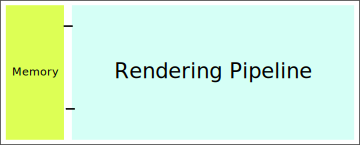
\includegraphics[width=12.5cm,keepaspectratio]{pics/pipeline/RenderingPipelineMemoryPipeline}}
	\end{picture}
\end{frame}

\begin{frame}
\frametitle{Zobrazovací řetězec}
	\begin{itemize}
		\item Zobrazovací řetěžec je rozdělen na 2 části - vektorovou a rastrovou.
    \item Dělícím prvkem je rasterizace.
	\end{itemize}
	\begin{picture}(320,250)
		\put(-25,100){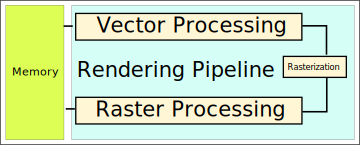
\includegraphics[width=12.5cm,keepaspectratio]{pics/pipeline/RenderingPipelineVectorRaster}}
	\end{picture}
\end{frame}


\begin{frame}
\frametitle{Vektorová část zobrazovacího řetězce}
	\begin{itemize}
		\item Vektorová část řetězce je složena z mnoha bloků.
    \item Některé bloky jsou programovatelné a některé vynechatelné.
	\end{itemize}
	\begin{picture}(320,250)
		\put(-25,60){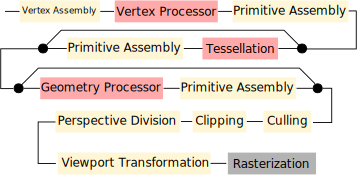
\includegraphics[width=12.5cm,keepaspectratio]{pics/pipeline/RenderingPipelineVector}}
	\end{picture}
\end{frame}

\begin{frame}
\frametitle{Vertex puller, vertex processor, primitive assembly}
	\begin{itemize}
		\item Vertex puller sestavuje vrcholy, vertex processro transformuje vrcholy, primitive assembly sestavuje primitiva.
	\end{itemize}
	\begin{picture}(320,250)
		\put(-25,100){
\includegraphics[width=12.5cm,keepaspectratio]{pics/pipeline/OpenGL460PipelineVertexShader}}
	\end{picture}
\end{frame}

\begin{frame}
\frametitle{Teselace}
	\begin{itemize}
		\item Tesselace je složena zde 2 programovatelných processorů.
	\end{itemize}
	\begin{picture}(320,250)
		\put(-25,100){
\includegraphics[width=12.5cm,keepaspectratio]{pics/pipeline/OpenGL460PipelineTessellationShaders}}
	\end{picture}
\end{frame}

\begin{frame}
\frametitle{Geometry processor, transform feedback}
	\begin{itemize}
		\item Geometry processor transformuje primitiva.
    \item Transform feedback může primitiva přeposlat zpět do bufferu.
	\end{itemize}
	\begin{picture}(320,250)
		\put(-25,100){
\includegraphics[width=12.5cm,keepaspectratio]{pics/pipeline/OpenGL460PipelineGeometryShader}}
	\end{picture}
\end{frame}

\begin{frame}
\frametitle{Culling, clipping}
	\begin{itemize}
		\item Těsně před raterizací se zahazují odvrácené trojúhelníky a zbylé se ořezávají pohledovým frustem.
	\end{itemize}
	\begin{picture}(320,250)
		\put(-25,100){
\includegraphics[width=12.5cm,keepaspectratio]{pics/pipeline/OpenGL460PipelineClipping}}
	\end{picture}
\end{frame}


\begin{frame}
\frametitle{Rasterizace a interpolace}
	\begin{itemize}
		\item Vertexy jsou před rasterizací popsány pomocí n-tice atributů
    \item Rasterizace produkuje fragmenty, pokud jejich střed leží uvnitř primitiva
    \item Po rasterizaci jsou tyto atributy vloženy do fragmetů pomocí interpolace
	\end{itemize}
	\begin{figure}[h]
		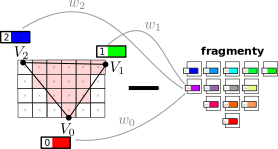
\includegraphics[width=10cm,keepaspectratio]{pics/pipeline/interpolace.pdf}
	\end{figure}
\end{frame}

\begin{frame}
\frametitle{Barycentrické koordináty}
	\begin{figure}[h]
		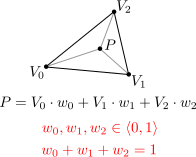
\includegraphics[width=10cm,keepaspectratio]{pics/pipeline/barycentrickekoordinaty.pdf}
	\end{figure}
\end{frame}

\begin{frame}
\frametitle{Perspektivní zkreslení}
	\begin{itemize}
		\item Vertex atributy se mohou interpolovat v rovině průmětny nebo v prostoru scény
    \item Aby se mohlo interpolovat v prostoru scény, musí se provést perspektivní korekce
      (v OpenGL automaticky/lze vypnout)
	\end{itemize}
	\begin{figure}[h]
		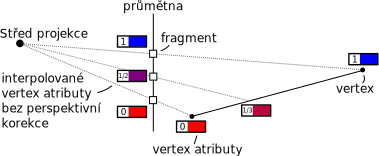
\includegraphics[width=10cm,keepaspectratio]{pics/pipeline/prespektivni_korekce.pdf}
	\end{figure}
\end{frame}


\begin{frame}
\frametitle{Rastrová část - rasterizace}
	\begin{picture}(320,250)
		\put(0,20){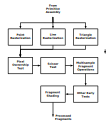
\includegraphics[width=7cm,keepaspectratio]{pics/pipeline/OpenGL460PipelineRaster}}
	\end{picture}
\end{frame}

\begin{frame}
\frametitle{Rastrová část - Per fragment operace}
	\begin{picture}(320,250)
		\put(-20,20){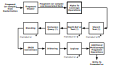
\includegraphics[width=12.5cm,keepaspectratio]{pics/pipeline/OpenGL460PipelineFragmentShader}}
	\end{picture}
\end{frame}



\begin{frame}
\frametitle{OpenGL 4.6 pipeline}
  \begin{figure}[h]
  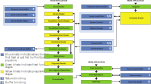
\includegraphics[width=10cm,keepaspectratio]{pics/pipeline/OpenGL460Pipeline}
  \end{figure}
\end{frame}


